\documentclass{article}
\usepackage{tikz}
\usepackage{amsmath}

\begin{document}

\begin{center}
\Large\textbf{A Mathematical Curiosity for 2025}
\end{center}

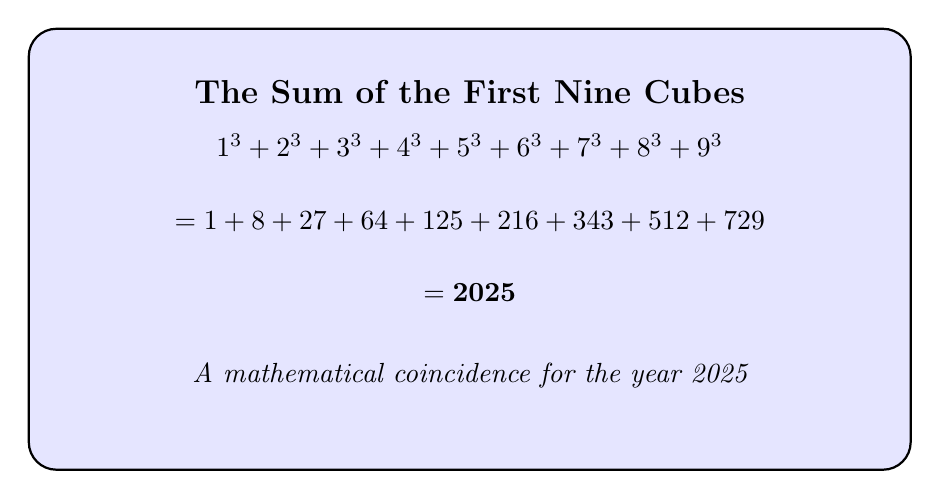
\begin{tikzpicture}[scale=0.8]
    % Create a decorative box
    \draw[rounded corners=10pt, thick, fill=blue!10] (-2,-1) rectangle (12,6);
    
    % Title
    \node[font=\large\bfseries] at (5,5) {The Sum of the First Nine Cubes};
    
    % Main equation
    \node[align=center] at (5,3) {
        $1^3 + 2^3 + 3^3 + 4^3 + 5^3 + 6^3 + 7^3 + 8^3 + 9^3$\\[0.5cm]
        $= 1 + 8 + 27 + 64 + 125 + 216 + 343 + 512 + 729$\\[0.5cm]
        $= \mathbf{2025}$
    };
    
    % Add a decorative note
    \node[font=\itshape] at (5,0.5) {A mathematical coincidence for the year 2025};
\end{tikzpicture}

\end{document} 
